\section{Theoretical Analysis}
\label{sec:analysis}

In this section, the circuit shown in Figure~\ref{fig:circuit} is analysed
theoretically, in terms of its time and frequency responses.

\subsection{Node Analysis for t<0}

In this section the circuit is analysed for t<0, according to the Figure~\ref{fig:nodes}, using the Node Method.\par

\begin{figure}[H] \centering
  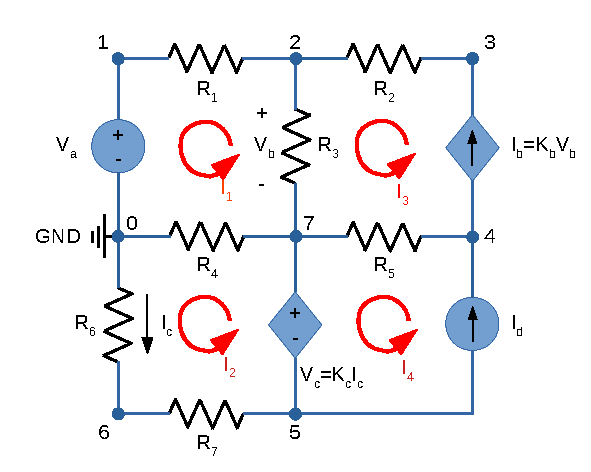
\includegraphics[width=0.7\linewidth]{MeshMethod.pdf}
  \caption{Mesh Currents Identification}
  \label{fig:MeshMethod}
\end{figure}

The system solved is shown below:\par

$$
\begin{bmatrix}
  1 & 0 & 0 & 0 & 0 & 0 & 0 \\
  G_{1} & -G_{1}-G_{2}-G_{3} & G_{2} & G_{3} & 0 & 0 & 0 \\
  0 & G_{2}+K_{b} & -G_{2} & -K_{b} & 0 & 0 & 0 \\
  0 & G_{3} & 0 & -G_{3}-G_{4}-G_{5} & G_{5} & G_{7} & -G_{7} \\
  0 & -K_{b} & 0 & K_{b}+G_{5} & -G_{5} & 0 & 0 \\
  0 & 0 & 0 & 0 & 0 & -G_{6}-G_{7} & G_{7} \\
  0 & 0 & 0 & 1 & 0 & K_{d}*G_{6} & -1
\end{bmatrix}
=
\begin{bmatrix}
  V_{1}\\
  V_{2}\\
  V_{3}\\
  V_{5}\\
  V_{6}\\
  V_{7}\\
  V_{8}
\end{bmatrix}
\begin{bmatrix}
  V_{s}\\
  0\\
  0\\
  0\\
  0\\
  0\\
  0
\end{bmatrix}
$$

The nodal voltages and the branch currents found by Octave to the system above
are displayed in Table~\ref{tab:volt1} and Table~\ref{tab:curr1}, respectively.\par

\begin{minipage}
\centering
\begin{table} [b]
  \begin{tabular}{|l|r|}
    \hline    
    {\bf Name} & {\bf Value [V]} \\ \hline
    $V_1$ & 5.12562725920 \\ \hline 
$V_2$ & 4.90389094213 \\ \hline 
$V_3$ & 4.44621543662 \\ \hline 
$V_4$ & 0.00000000000 \\ \hline 
$V_5$ & 4.93496307069 \\ \hline 
$V_6$ & 5.63581571238 \\ \hline 
$V_7$ & -1.97571911988 \\ \hline 
$V_8$ & -2.98274501015 \\ \hline 

  \end{tabular}
  \caption{Nodal voltages, expressed in Volts, when t<0}
  \label{tab:volt1}
\end{table}
\end{minipage}
\begin{minipage}
\begin{table} [b]
  \begin{tabular}{|l|r|}
    \hline    
    {\bf Name} & {\bf Ampere [A]} \\ \hline
    $I_1$ & 0.00021612262 \\ \hline 
$I_2$ & -0.00022637255 \\ \hline 
$I_3$ & -0.00001024993 \\ \hline 
$I_4$ & 0.00119458862 \\ \hline 
$I_5$ & -0.00022637255 \\ \hline 
$I_6$ & 0.00097846600 \\ \hline 
$I_7$ & 0.00097846600 \\ \hline 
$I_b$ & -0.00022637255 \\ \hline 
$I_c$ & -0.00000000000 \\ \hline 
$I_{V_d}$ & 0.00097846600 \\ \hline 
$I_{V_s}$ & 0.00021612262 \\ \hline 

  \end{tabular}
  \caption{Currents, expressed in Ampere, when t<0}
  \label{tab:curr1}
\end{table}
\end{minipage}

The results obtained show the behaviour of the circuit before $V_s$ is oscilating.

\subsection{Node Analysis for $V_s$=0}

Throughout this section, it is computed the equivalent resistance, $R_{eq}$, from
the capacitor terminals. To achieve that, we make $V_{s}=0$ and replace the capacitor
with the voltage source $V_{x}=V_{6}-V_{8}$, where $V_6$ and $V_8$ are the voltages
in nodes 6 and 8, respectively.\par
The matricial form of the system solved is shown below:\par

$$
\begin{bmatrix}
  1 & 0 & 0 & 0 & 0 & 0 & 0 \\
  G_{1} & -G_{1}-G_{2}-G_{3} & G_{2} & G_{3} & 0 & 0 & 0 \\
  0 & G_{2}+K_{b} & -G_{2} & -K_{b} & 0 & 0 & 0 \\
  0 & 0 & 0 & 1 & 0 & K_{d}*G_{6} & -1 \\
  0 & 0 & 0 & 0 & 1 & 0 & -1 \\
  0 & 0 & 0 & 0 & 0 & -G_{6}-G_{7} & G_{7} \\
  G_{4} & G_{3} & 0 & -G_{3}-G_{4} & 0 & G_{6}+G_{7} & -G_{7}
\end{bmatrix}
=
\begin{bmatrix}
  V_{1}\\
  V_{2}\\
  V_{3}\\
  V_{5}\\
  V_{6}\\
  V_{7}\\
  V_{8}
\end{bmatrix}
\begin{bmatrix}
  V_{s}\\
  0\\
  0\\
  0\\
  V_{x}\\
  0\\
  0
\end{bmatrix}
$$

In Table~\ref{tab:volt2}, the results from the matricial system are presented.\par

\begin{table} [H]
  \centering
  \begin{tabular}{|l|r|}
    \hline    
    {\bf Name} & {\bf Value [V]} \\ \hline
    $V_1$ & 0.00000000000 \\ \hline 
$V_2$ & 0.00000000000 \\ \hline 
$V_3$ & 0.00000000000 \\ \hline 
$V_4$ & 0.00000000000 \\ \hline 
$V_5$ & 0.00000000000 \\ \hline 
$V_6$ & 8.61856072253 \\ \hline 
$V_7$ & 0.00000000000 \\ \hline 
$V_8$ & 0.00000000000 \\ \hline 

  \end{tabular}
  \caption{Nodal voltages, expressed in Volts, when $V_s$=0}
  \label{tab:volt2}
\end{table}

By creating a Thèvenin equivalent circuit, as seen from the voltage source's
terminals ($V_x$) and solving this matricial system, one can compute the current
$I_x$ passing on the voltage source $V_x$, using the formula:\par

\begin{equation}
  I_x = G_5 * (V_5 - V_6) - K_b * (V_2 - V_5).
  \label{eq:Ix}
\end{equation}

In doing so, one can compute the equivalent resistance, $R_{eq}$, by dividing the
voltage $V_x$ over the current $I_x$.

\begin{equation}
  R_{eq} = \frac{V_x}{I_x}.
  \label{eq:R_eq}
\end{equation}

\begin{table} [H]
  \centering
  \begin{tabular}{|l|r|}
    \hline    
    {\bf Name} & {\bf Value} \\ \hline
    $I_x$ & -0.00278375998 A \\ \hline 
$V_x$ & 8.61856072253 V \\ \hline 
$R_{eq}$ & 3096.01431108000 Ohm \\ \hline 

  \end{tabular}
  \caption{Equivalent resistance, voltage $V_x$ and current $I_x$, when $V_s$=0}
  \label{tab:req}
\end{table}








The circuit consists of a single V-R-C loop where a current $i(t)$ circulates. The
voltage source $v_I(t)$ drives its input, and the output voltage $v_O(t)$ is taken from
the capacitor terminals. Applying the Kirchhoff Voltage Law (KVL), a single
equation for the single loop in the circuit can be written as

\begin{equation}
  Ri(t) + v_O(t) = v_I(t).
  \label{eq:kvl}
\end{equation}

Because $v_O$ is the voltage between capacitor C's plates, it is related to the
current $i$ by
\begin{equation}
  i(t) = C\frac{dv_O}{dt}.
\end{equation}

Hence, Equation~(\ref{eq:kvl}) can be rewritten as
\begin{equation}
  RC\frac{dv_O}{dt} + v_O(t) = v_I.
  \label{eq:kvl2}
\end{equation}

Equation~(\ref{eq:kvl2}) is a linear differencial equation whose solution is a
superposition of a natural solution $v_{On}$ and a forced solution $v_{Of}$:

\begin{equation}
  v_O(t) = v_{On}(t) + v_{Of}(t).
  \label{eq:vo_sol}
\end{equation}

As learned in the theory classes the natural solution is of the form
\begin{equation}
  v_{On}(t) = Ae^{-\frac{t}{RC}},
  \label{eq:vo_nat}
\end{equation}
where $A$ is an integration constant.

The forced solution is of the form given in Equation~(\ref{eq:vo_for}) and is
illustrated in Figure~\ref{fig:forced}.

\begin{equation}
  V_{Of}(t) = |\bar{V}_{Of}| cos(\omega t + \angle \bar{V}_{Of}),
  \label{eq:vo_for}
\end{equation}

\lipsum[1-1]


\begin{figure}[h] \centering
\includegraphics[width=0.8\linewidth]{forced.eps}
\caption{Forced sinusoidal response.}
\label{fig:forced}
\end{figure}

\section{Frequency response}

\lipsum[1-1]


